\documentclass[journal,12pt,twocolumn]{IEEEtran}

\usepackage{setspace}
\usepackage{gensymb}

\singlespacing


\usepackage[cmex10]{amsmath}

\usepackage{amsthm}

\usepackage{mathrsfs}
\usepackage{txfonts}
\usepackage{stfloats}
\usepackage{bm}
\usepackage{cite}
\usepackage{cases}
\usepackage{subfig}

\usepackage{longtable}
\usepackage{multirow}

\usepackage{enumitem}
\usepackage{mathtools}
\usepackage{steinmetz}
\usepackage{tikz}
\usepackage{circuitikz}
\usepackage{verbatim}
\usepackage{tfrupee}
\usepackage[breaklinks=true]{hyperref}
\usepackage{graphicx}
\usepackage{tkz-euclide}

\usetikzlibrary{calc,math}
\usepackage{listings}
    \usepackage{color}                                            %%
    \usepackage{array}                                            %%
    \usepackage{longtable}                                        %%
    \usepackage{calc}                                             %%
    \usepackage{multirow}                                         %%
    \usepackage{hhline}                                           %%
    \usepackage{ifthen}                                           %%
    \usepackage{lscape}     
\usepackage{multicol}
\usepackage{chngcntr}

\DeclareMathOperator*{\Res}{Res}

\renewcommand\thesection{\arabic{section}}
\renewcommand\thesubsection{\thesection.\arabic{subsection}}
\renewcommand\thesubsubsection{\thesubsection.\arabic{subsubsection}}

\renewcommand\thesectiondis{\arabic{section}}
\renewcommand\thesubsectiondis{\thesectiondis.\arabic{subsection}}
\renewcommand\thesubsubsectiondis{\thesubsectiondis.\arabic{subsubsection}}


\hyphenation{op-tical net-works semi-conduc-tor}
\def\inputGnumericTable{}                                 %%

\lstset{
%language=C,
frame=single, 
breaklines=true,
columns=fullflexible
}
\begin{document}


\newtheorem{theorem}{Theorem}[section]
\newtheorem{problem}{Problem}
\newtheorem{proposition}{Proposition}[section]
\newtheorem{lemma}{Lemma}[section]
\newtheorem{corollary}[theorem]{Corollary}
\newtheorem{example}{Example}[section]
\newtheorem{definition}[problem]{Definition}

\newcommand{\BEQA}{\begin{eqnarray}}
\newcommand{\EEQA}{\end{eqnarray}}
\newcommand{\define}{\stackrel{\triangle}{=}}
\bibliographystyle{IEEEtran}
\providecommand{\mbf}{\mathbf}
\providecommand{\pr}[1]{\ensuremath{\Pr\left(#1\right)}}
\providecommand{\qfunc}[1]{\ensuremath{Q\left(#1\right)}}
\providecommand{\sbrak}[1]{\ensuremath{{}\left[#1\right]}}
\providecommand{\lsbrak}[1]{\ensuremath{{}\left[#1\right.}}
\providecommand{\rsbrak}[1]{\ensuremath{{}\left.#1\right]}}
\providecommand{\brak}[1]{\ensuremath{\left(#1\right)}}
\providecommand{\lbrak}[1]{\ensuremath{\left(#1\right.}}
\providecommand{\rbrak}[1]{\ensuremath{\left.#1\right)}}
\providecommand{\cbrak}[1]{\ensuremath{\left\{#1\right\}}}
\providecommand{\lcbrak}[1]{\ensuremath{\left\{#1\right.}}
\providecommand{\rcbrak}[1]{\ensuremath{\left.#1\right\}}}
\theoremstyle{remark}
\newtheorem{rem}{Remark}
\newcommand{\sgn}{\mathop{\mathrm{sgn}}}
\providecommand{\abs}[1]{\left\vert#1\right\vert}
\providecommand{\res}[1]{\Res\displaylimits_{#1}} 
\providecommand{\norm}[1]{\left\lVert#1\right\rVert}
%\providecommand{\norm}[1]{\lVert#1\rVert}
\providecommand{\mtx}[1]{\mathbf{#1}}
\providecommand{\mean}[1]{E\left[ #1 \right]}
\providecommand{\fourier}{\overset{\mathcal{F}}{ \rightleftharpoons}}
%\providecommand{\hilbert}{\overset{\mathcal{H}}{ \rightleftharpoons}}
\providecommand{\system}{\overset{\mathcal{H}}{ \longleftrightarrow}}
	%\newcommand{\solution}[2]{\textbf{Solution:}{#1}}
\newcommand{\solution}{\noindent \textbf{Solution: }}
\newcommand{\cosec}{\,\text{cosec}\,}
\providecommand{\dec}[2]{\ensuremath{\overset{#1}{\underset{#2}{\gtrless}}}}
\newcommand{\myvec}[1]{\ensuremath{\begin{pmatrix}#1\end{pmatrix}}}
\newcommand{\mydet}[1]{\ensuremath{\begin{vmatrix}#1\end{vmatrix}}}
\numberwithin{equation}{subsection}
\makeatletter
\@addtoreset{figure}{problem}
\makeatother
\let\StandardTheFigure\thefigure
\let\vec\mathbf
\renewcommand{\thefigure}{\theproblem}
\def\putbox#1#2#3{\makebox[0in][l]{\makebox[#1][l]{}\raisebox{\baselineskip}[0in][0in]{\raisebox{#2}[0in][0in]{#3}}}}
     \def\rightbox#1{\makebox[0in][r]{#1}}
     \def\centbox#1{\makebox[0in]{#1}}
     \def\topbox#1{\raisebox{-\baselineskip}[0in][0in]{#1}}
     \def\midbox#1{\raisebox{-0.5\baselineskip}[0in][0in]{#1}}
\vspace{3cm}
\title{Assignment 1}
\author{Sowmya Bandi}
\maketitle
\newpage
\bigskip
\renewcommand{\thefigure}{\theenumi}
\renewcommand{\thetable}{\theenumi}
Download all python codes from 
\begin{lstlisting}
https://github.com/sowmyabandi882/ASSIGNMNT/blob/main/Asignment%201/Assignment1.py
\end{lstlisting}
%
and latex-tikz codes from 
%
\begin{lstlisting}
https://github.com/sowmyabandi882/ASSIGNMNT/blob/main/Asignment%201/main.tex
\end{lstlisting}
%
\section{Question No.2.7}
\item In $\triangle ABC$,  $a = 8, \angle B = 45^{\degree}$ and $c-b = 3.5$.
Sketch $\triangle ABC$.

 
%
%
\section{SOLUTION}
 
Given,
\begin{align}
\ BC = 8,
\angle B = 45^{\degree}$ and
\ AB-AC = 3.5$
\end{align}


let the vertices of $\triangle ABC$ and D be
\begin{align}
\vec{A} = \myvec{p\\q}, \vec{B} = \myvec{0\\0}, \vec{C} = \myvec{a\\0},\vec{D} = \myvec{p\\0}
\end{align}


we have,
\begin{align}
c-b=3.5
\\
\implies c=3.5+b
\end{align}

From $\triangle ABC$,we use the law of cosines: 
\begin{align}
b^2=a^2 + c^2 - 2ac CosB
\\
b^2=(8)^2 + (3.5+b)^2 - 2(8)(3.5+b)Cos45
\\
b^2=64 + 12.25 + 7b + b^2 - 29.4168 - 8.4b
\\
\implies 0=46.83 - 1.4b
\\
\implies b=\frac{46.83}{1.4}
\\
\implies b=33.45
\end{align}

From 2.0.3,
\begin{align}
c-b=3.5
\\
\implies c - 33.45=3.5
\\
c=36.95
\end{align}
Then,
\begin{align}
AB = \norm{\vec{A}-\vec{B}} = \norm{A}^2=c^2
\\
BC = \norm{\vec{C}-\vec{B}}^2 = \norm{C}^2= a^2
\\
AC = \norm{\vec{A}-\vec{C}}^2 = b^2
\end{align}
From 2.0.16,
\begin{align}
\implies b^2=\norm{\vec{A}-\vec{C}}^2=({\vec{A}-\vec{C}})^T ({\vec{A}-\vec{C}})
\\
b^2= \vec{A}^T\vec{A}+\vec{C}^T\vec{C}-\vec{A}^T\vec{C} - \vec{A}\vec{C}^T
\\
b^2= \norm{\vec{A}}^2 + \norm{\vec{C}}^2 - 2\vec{C}^T\vec{A} 
\\
b^2= a^2 + c^2 - 
\end{align}
yielding,
\begin{align}
p=\frac{a^2 + c^2 - b^2}{2c}
\\
p=\frac{(8)^2 + (36.95)^2 - (33.45)^2}{2(36.95)}
\\
p=\frac{310.9}{73.9}
\\
p=4.2
\end{align}
From 2.0.14,
\begin{align}
\norm{A}^2=c^2=p^2 +  (2q)^2
\\
q^2=\frac{c^2 - p^2}{4}
\\
q^2= \frac{(36.95)^2 - (4.2)^2}{4}
\\
q^2= 336.91
\\
q= \pm 18.35 
\end{align}
As we consider $\triangle ABC$ in first quadrant.we consider $q$ = 18.35
\\
Therefore,$q$ = 18.35
\\
so,the vertices of $\triangle ABC$ and D are
\begin{align}
\vec{A} = \myvec{4.2\\18.35}, \vec{B} = \myvec{0\\0}, \vec{C} = \myvec{8\\0},\vec{D} = \myvec{4.2\\0}
\end{align}

\tikzset{every picture/.style={line width=0.75pt}} %set default line width to 0.75pt        

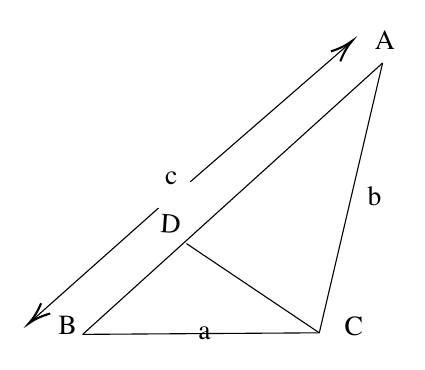
\begin{tikzpicture}[x=0.75pt,y=0.75pt,yscale=-1,xscale=1]
%uncomment if require: \path (0,300); %set diagram left start at 0, and has height of 300

%Straight Lines [id:da5097063893301796] 
\draw    (280.5,229.75) -- (166.5,230.5) ;
%Straight Lines [id:da7850802292038823] 
\draw    (311,99.75) -- (166.5,230.5) ;
%Straight Lines [id:da6365544413224928] 
\draw    (311,99.75) -- (280.5,229.75) ;
%Straight Lines [id:da7929091978862834] 
\draw    (216.5,186.75) -- (280.5,229.75) ;
%Straight Lines [id:da7712407683082501] 
\draw    (218.33,157) -- (293.96,91.31) -- (294.88,90.45) ;
\draw [shift={(296.33,89.08)}, rotate = 496.76] [color={rgb, 255:red, 0; green, 0; blue, 0 }  ][line width=0.75]    (10.93,-3.29) .. controls (6.95,-1.4) and (3.31,-0.3) .. (0,0) .. controls (3.31,0.3) and (6.95,1.4) .. (10.93,3.29)   ;
%Straight Lines [id:da9275356671665713] 
\draw    (203,169.67) -- (141.99,223.92) ;
\draw [shift={(140.5,225.25)}, rotate = 318.35] [color={rgb, 255:red, 0; green, 0; blue, 0 }  ][line width=0.75]    (10.93,-3.29) .. controls (6.95,-1.4) and (3.31,-0.3) .. (0,0) .. controls (3.31,0.3) and (6.95,1.4) .. (10.93,3.29)   ;

% Text Node
\draw (203.29,171.38) node [anchor=north west][inner sep=0.75pt]  [rotate=-3.95] [align=left] {D};
% Text Node
\draw (306,83) node [anchor=north west][inner sep=0.75pt]   [align=left] {A};
% Text Node
\draw (291.5,221) node [anchor=north west][inner sep=0.75pt]   [align=left] {C};
% Text Node
\draw (153.5,220.5) node [anchor=north west][inner sep=0.75pt]   [align=left] {B};
% Text Node
\draw (205,151) node [anchor=north west][inner sep=0.75pt]   [align=left] {c};
% Text Node
\draw (221,225.5) node [anchor=north west][inner sep=0.75pt]   [align=left] {a};
% Text Node
\draw (302.5,158) node [anchor=north west][inner sep=0.75pt]   [align=left] {b};


\end{tikzpicture}
\\
Fig. 2.1:$\triangle ABC$
\end{document}

